\documentclass[12pt,a4paper,twoside]{article}
\usepackage[utf8]{inputenc}
\usepackage[spanish]{babel}
\usepackage{amsmath}
\usepackage{amsfonts}
\usepackage{amssymb}
\usepackage{graphicx}
\usepackage[left=2cm,right=2cm,top=2cm,bottom=2cm]{geometry}
\author{Yoleivys Delgado}
\title{\textbf{Evaluación 2}}
\begin{document}
\maketitle
En este documento se presentan los ejercicios propuestos y resueltos de la evaluacion 2 del curso de programación Fortran.
\section{Ejercicio 1 }
Se proporciona el siguiente código, que utiliza una función en Fortran 90 para la Serie de Maclaurin function exptaylor(x,n)para aproximar la función exponencial $f(x) = exp(x)$, en el punto x=1, utilizando n=20 términos de la serie.Ver figura (\ref{fig:figura1})
Copia el programa y verifica que datos produce y explica los resultados de la salida.\\

Resultado 
\begin{verbatim}
 x =    1.0000000000000000     
 exp_true  =    2.7182818284590451     
 exptaylor =    2.7182818284590455     
 error     =    4.4408920985006262E-016
\end{verbatim}

Aproximacion calculada con un error muy pequeño 
\begin{figure}
  \begin{verbatim}
!taylor.f90

program taylor

    implicit none                  
    real (kind=8) :: x, exp_true, y
    real (kind=8), external :: exptaylor
    integer :: n

    n = 20               ! number of terms to use
    x = 1.0
    exp_true = exp(x)
    y = exptaylor(x,n)   ! uses function below
    print *, "x = ",x
    print *, "exp_true  = ",exp_true
    print *, "exptaylor = ",y
    print *, "error     = ",y - exp_true

end program taylor

!==========================
function exptaylor(x,n)
!==========================
    implicit none

    ! function arguments:
    real (kind=8), intent(in) :: x
    integer, intent(in) :: n
    real (kind=8) :: exptaylor

    ! local variables:
    real (kind=8) :: term, partial_sum
    integer :: j

    term = 1.
    partial_sum = term

    do j=1,n
        ! j'th term is  x**j / j!  which is the previous term times x/j:
        term = term*x/j   
        ! add this term to the partial sum:
        partial_sum = partial_sum + term   
        enddo
     exptaylor = partial_sum  ! this is the value returned
end function exptaylor

! --------  End -------------
  \end{verbatim}
\caption{Cogigo Fortran del ejercicio 1 }
\label{fig:figura1}
\end{figure}

\section{Ejercicio 2}
Apoyado en el código de la función  exptaylor(x,n), diseña ahora una nueva subrutina en Fortran 90 para calcular la aproximación de la función en un rango de x, digamos de x0=0.0 a x1=10.0, evaluando en un número de puntos npts=100. Es decir la función exptaylor(x,n) admite ahora un arreglo x de dimensión npts y un entero n que es el orden de la aproximación.\\
Se pide que aproximes la función $f(x)= exp(x)$, utilizando sólo los primeros n términos de la serie $(n=1,3,5,7,...,15 )$, es decir crea las siguientes funciones de datos f1, f3, f5, f7, ..., f15 y guarda los datos en un archivo para contrastar que tan bien se aproxima la función exp(x) si sólo usamos f1, f3, f5, f7, ..., f15. Usando Gnuplot, gráfica la función real exp(x), y sus aproximaciones f1, f3, f5, f7, ..., f15. No es necesario calcular el error. \\
La figura obtenido en este ejercicio se muestra en la figura (\ref{fig:figura2}). El codigo fortran y gnuplot de este ejercicio se muestran en las (\ref{fig:figura3})y(\ref{fig:figura4})
\begin{figure}[h]
\centering
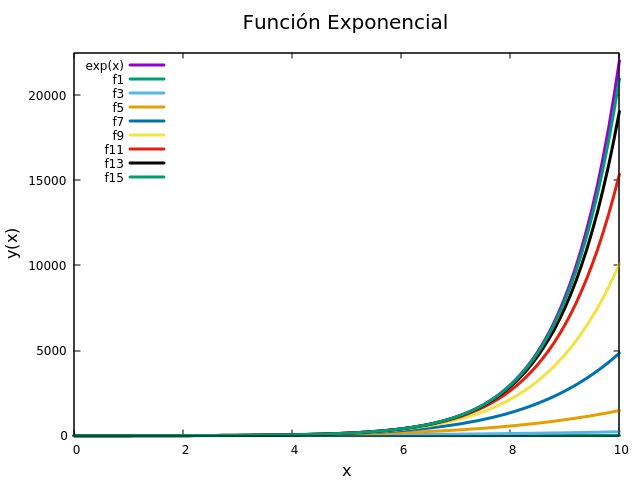
\includegraphics[width=10cm]{Ejercicio2.png} 
\caption{f(x)= exp(x) y sus primeras aproximaciones }
\label{fig:figura2}
\end{figure}

\begin{figure}[h]
\begin{verbatim}
set title 'Función Exponencial'
set title font ",15" norotate
set xlabel "x"
set xlabel font "Verdana,12"
set ylabel "y(x)"
set ylabel font "Verdana,12"
set style data line
set xrange [0:10]
set yrange [0:22500]
set key left
plot [0:10] exp(x) title "exp(x)" with lines lt 1 linewidth 3,\
"ejercicio2.txt" index 0 using 1:2  lt 2 linewidth 3  title "f1",\
"ejercicio2.txt" index 1 using 1:2  lt 3 linewidth 3 title "f3",\
"ejercicio2.txt" index 2 using 1:2  lt 4 linewidth 3 title "f5",\
"ejercicio2.txt" index 3 using 1:2  lt 6 linewidth 3 title "f7",\
"ejercicio2.txt" index 4 using 1:2  lt 5 linewidth 3 title "f9",\
"ejercicio2.txt" index 5 using 1:2  lt 7 linewidth 3 title "f11",\
"ejercicio2.txt" index 6 using 1:2  lt 16 linewidth 3 title "f13",\
"ejercicio2.txt" index 7 using 1:2  lt 10 linewidth 3 title "f15"
\end{verbatim}
\caption{Codigo gnuplot de la gráfica de la figura 2}
\label{fig:figura3}
\end{figure}

\begin{figure}
\begin{verbatim}
program functionexp

    implicit none                  
    real (kind=8) :: x2, exp2,exp3
    integer :: n2, npts,i,k,s

    s = 15               ! number of terms to use
    npts=100
    
    open (1,file ='ejercicio2.txt', status ='unknown')

    do k=1,s,2
       n2 = k
        do i=0,npts
        x2 = i*0.1
       
        
       call fun_exp(x2,n2,exp2)

       exp3=exp2
       write (1,*) x2, exp3
      
         end do
         write (1,*) ''
         write (1,*) ''
         
     end do
     
   close (1)

  end program functionexp

  
!==========================
subroutine fun_exp(x,n,exp)
!==========================
    implicit none

    ! subroutine arguments:
    real (kind=8), intent(in) :: x
    integer, intent(in) :: n
    real (kind=8), intent (out) :: exp
    

    ! local variables:
    real (kind=8) :: term, partial_sum
    integer :: j
    
    !inicialition 
    term = 1.
    partial_sum = term
    
    do j=1,n
        ! j'th term is  x**j / j!  which is the previous term times x/j:
        term = term*x/j   
        ! add this term to the partial sum:
        partial_sum = partial_sum + term   
     enddo
       exp = partial_sum  ! this is the value returned
       
end subroutine  fun_exp

! --------  End -------------

\end{verbatim}
\caption{Codigo Fortran de la gráfica de la figura 2}
\label{fig:figura4}
\end{figure}

\section{Ejercicio 3}

 Modifica tu código para ahora aproximar la función $f(x) = sin(x)$, en el intervalo x = - 3 pi a x = 3 pi. Realiza una actividad similar a la anterior. Deberás obtener una gráfica parecida a la que aparece arriba al principio de esta Evaluación.
 La grafica obtenida de este ejercicio se muestra en la figura (\ref{fig:figura5}) y los codigos Fortran y gnuplot en las figuras (\ref{fig:figura6}) y (\ref{fig:figura7}.

\begin{figure}[h]
\centering
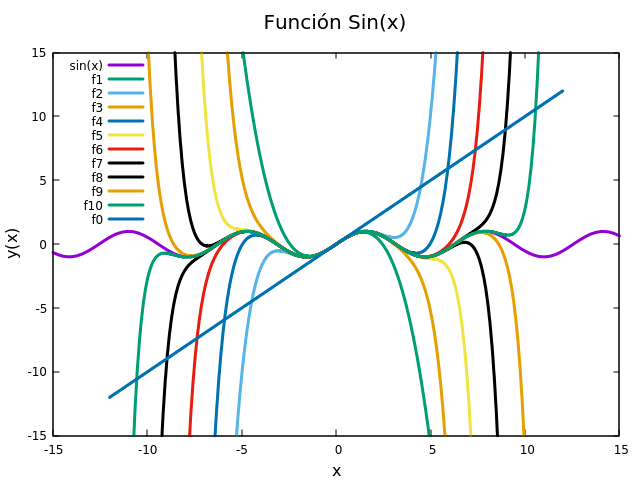
\includegraphics[width=10cm]{Ejercicio3.png} 
\caption{f(x) = sin(x) y sus primeras aproximaciones}
\label{fig:figura5}
\end{figure}

\begin{figure}[h]
\begin{verbatim}
set title 'Función Sin(x)'
set title font ",15" norotate
set xlabel "x"
set xlabel font "Verdana,12"
set ylabel "y(x)"
set ylabel font "Verdana,12"
set style data line
set xrange [-15:15]
set yrange [-15:15]
set key left
plot [-15:15] sin(x) title "sin(x)" with lines lt 1 linewidth 3,\
"ejercicio3.txt" index 0 using 1:2  lt 2 linewidth 3  title "f1",\
"ejercicio3.txt" index 1 using 1:2  lt 3 linewidth 3 title "f2",\
"ejercicio3.txt" index 2 using 1:2  lt 4 linewidth 3 title "f3",\
"ejercicio3.txt" index 3 using 1:2  lt 6 linewidth 3 title "f4",\
"ejercicio3.txt" index 4 using 1:2  lt 5 linewidth 3 title "f5",\
"ejercicio3.txt" index 5 using 1:2  lt 7 linewidth 3 title "f6",\
"ejercicio3.txt" index 6 using 1:2  lt 16 linewidth 3 title "f7",\
"ejercicio3.txt" index 7 using 1:2  lt -1 linewidth 3 title "f8",\
"ejercicio3.txt" index 8 using 1:2  lt 4 linewidth 3 title "f9",\
"ejercicio3.txt" index 9 using 1:2  lt 10 linewidth 3 title "f10",\
"ejercicio3.txt" index 0 using 1:3  lt 6 linewidth 3 title "f0"
\end{verbatim}
\caption{Codigo gnuplot de la gráfica de la figura 5}
\label{fig:figura6}
\end{figure}


\begin{figure}[h]
\begin{verbatim}
program fun_seno

    implicit none                  
    real (kind=8) :: x2, sin_x2,sin_x3,y
    integer :: n2, npts,i,s,k
    integer,parameter :: Pi=3.1416

    s = 10               ! number of terms to use
    npts=720
    
    open (3,file ='ejercicio3.txt', status ='unknown')

    do k=1,s     
       
       n2=k
        do i=-npts,npts
        
        x2 = real(i)*Pi/180.
        y=x2
       call fun_sin (x2,n2,sin_x2)

       sin_x3=sin_x2

       write (3,*) x2, sin_x3, y
         end do
         write (3,*) ''
         write (3,*) ''
     end do
   close (1)

  end program fun_seno

  
!==========================
subroutine fun_sin(x,n,sin_x)
!==========================
    implicit none

    ! subroutine arguments:
    real (kind=8), intent(in) :: x
    integer, intent(in) :: n
    real (kind=8), intent (out) :: sin_x
    

    ! local variables:
    real (kind=8) :: term, partial_sum
    integer :: j
    
    !inicialition 
    term = x
    partial_sum = term
    
    do j=1,n
       ! j'th term is  x**2j+1 / 2j+1!  which is the previous term
       ! times x**2/(2*j*(2*j+1)
        term = (-1**j)*(term*x*x)/(2*j*(2*j+1)) 
        ! add this term to the partial sum:
        partial_sum = partial_sum + term  
     enddo
     
      sin_x = partial_sum   ! this is the value returned

    
end subroutine  fun_sin

! --------  End ------------
\end{verbatim}
\caption{Codigo Fortran de la gráfica de la figura 5}
\label{fig:figura7}
\end{figure}
\end{document}